\chapter{Introduction}
\section{Multipath in Aeronautical Telemetry}
Multipath interference is one of the dominant causes for link loss in aeronautical telemetry.
Strong multipath interference occurs in aeronautical telemetry when the transmitted signal is received from multiple paths because a test article is in a low elevation angle scenario as shown in Figure \ref{fig:multipath}.
Multipath propagation is modeled as linear, time-invariant system with a finite impulse response.
Equalizers have been studied to combat multipath interference in aeronautical telemetry \cite{rice-afran-saquib:2014,rice-afran-saquib-cole-rhodes-moazzami:2014}.

There are two types of equalizers, blind and data-aided.
Blind equalizers combat multipath using known properties of the transmitted signal but no knowledge of the data or multipath channel.
Data-aided equalizers require knowing something about the received signal.
One method of providing data that can be used in data-aided equalization is for the transmitter to periodically insert a known bit sequence called a ``pilot'' into the data stream.
The receiver compares the received signal with a locally stored copy to estimate parameters such as multipath channels, frequency offsets, phase offsets and noise variance.
Data-aided equalizers are finite-length impulse response (FIR) filters. The impulse response of the equalizer filter is computed based on the estimated channel better mitigate multipath.
\begin{figure}
	\centering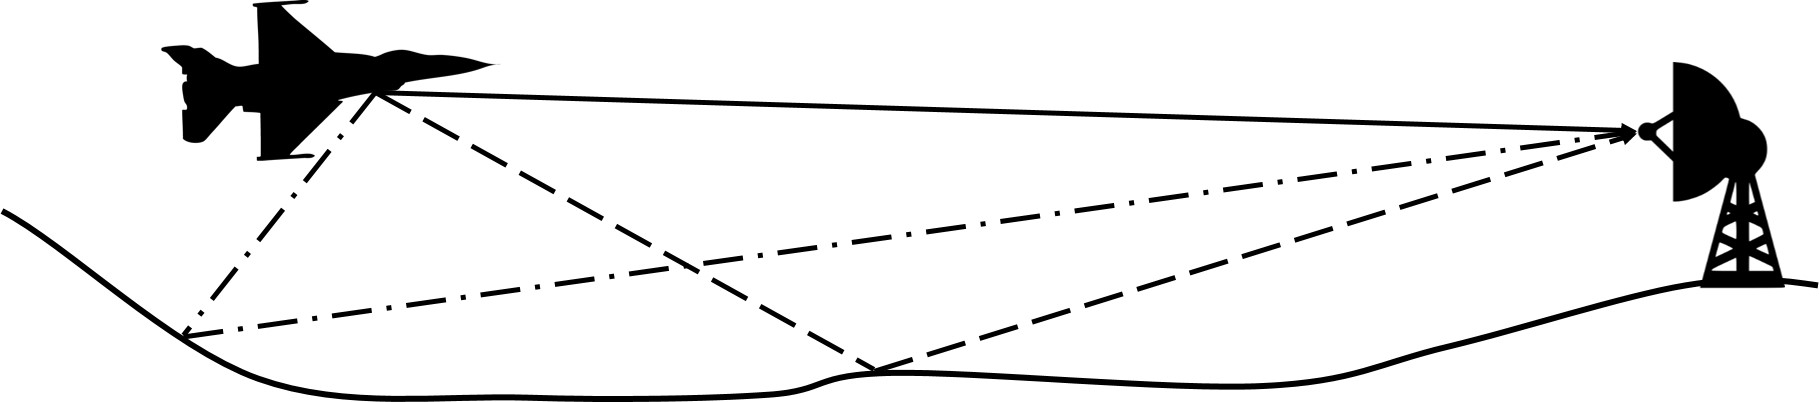
\includegraphics[width=12.11in/100*50]{figures/intro/Picture1.jpg}
	\caption{Multipath can occur when a signal is received multiple paths like line-of-sight or ground bounce or reflections.}
	\label{fig:multipath}
\end{figure}
\section{Problem Statement}
The signal processing for a digital communications system with data-aided equalizers is computationally heavy.
Algorithms implemented in a high powered Central Processing Unit (CPU) can not processing in real-time.
Graphic Processing Units (GPUs) can be used to perform real-time processing because of their massively parallel architecture.

This thesis studies how signal processing can be reformulated to run quickly and efficiently in GPUs.
Processing signals in batches to introduce more parallelism.
Optimized libraries harness GPU resources to make signal processing implementation relatively easy and extremely fast.
If algorithms can be reformulated to used matrix/vector multiplication, solving linear systems of equations, or the Fast Fourier Transform, GPUs can provide vast speed ups.

\section{Organization}
Chapter \ref{chap:equations} shows the equations for these block diagrams.
Chapter \ref{chap:gpu} will shed some light on signal processing in GPUs.
Chapter \ref{chap:equalizers_in_gpus} will illustrate how the five equalizers are implemented in GPUs.
Chapter \ref{chap:final_summary} will summarize.